\begin{savequote}[120mm]
Up ahead in the distance \\
I saw a shimmering light \\
My head grew heavy and my sight grew dim \\
I had to stop for the night
\qauthor{--- Eagles, \textit{Hotel California}, 1977}
\end{savequote}


\chapter{The Quark template}
\label{chapter1}
\thispagestyle{fancy}

\textit{Lorem ipsum dolor sit amet, consectetuer adipiscing elit. Ut purus elit, vestibulum ut, plac- erat ac, adipiscing vitae, felis. Curabitur dictum gravida mauris. Nam arcu libero, nonummy eget, consectetuer id, vulputate a, magna. Donec vehicula augue eu neque. Pellentesque habitant morbi tristique senectus et netus et malesuada fames ac turpis egestas. Mauris ut leo. Cras viverra metus rhoncus sem. Nulla et lectus vestibulum urna fringilla ultrices. Phasellus eu tellus sit amet tortor gravida placerat. Integer sapien est, iaculis in, pretium quis, viverra ac, nunc. Praesent eget sem vel leo ultrices bibendum. Aenean faucibus. Morbi dolor nulla, malesuada eu, pulvinar at, mollis ac, nulla. Curabitur auctor semper nulla. Donec varius orci eget risus. Duis nibh mi, congue eu, accumsan eleifend, sagittis quis, diam. Duis eget orci sit amet orci dignissim rutrum.}

%{\chapHeadFont

\paragraph{Paragraph 1}

Lorem ipsum dolor sit amet, consectetuer adipiscing elit. Ut purus elit, vestibulum ut, plac- erat ac, adipiscing vitae, felis. Curabitur dictum gravida mauris. Nam arcu libero, nonummy eget, consectetuer id, vulputate a, magna. Donec vehicula augue eu neque. Pellentesque habitant morbi tristique senectus et netus et malesuada fames ac turpis egestas. Mauris ut leo. Cras viverra metus rhoncus sem. Nulla et lectus vestibulum urna fringilla ultrices. Phasellus eu tellus sit amet tortor gravida placerat. Integer sapien est, iaculis in, pretium quis, viverra ac, nunc. Praesent eget sem vel leo ultrices bibendum. Aenean faucibus. Morbi dolor nulla, malesuada eu, pulvinar at, mollis ac, nulla. Curabitur auctor semper nulla. Donec varius orci eget risus. Duis nibh mi, congue eu, accumsan eleifend, sagittis quis, diam. Duis eget orci sit amet orci dignissim rutrum.



\section{Bibliography, citation and hyperlink}

\subsection{hyperlink}

Use the command \texttt{secref} to refer to sections such as the \secref{sectionA}. Use the command \texttt{secref} to refer to sections such as the \chapref{chapter1}. There also exists the commands \texttt{appref, remref, figref, tabref} for appendices, remarks, figures and tables.

\subsection{Citations}

Citations and notes are put in the margin. To place a note use the command  \texttt{notenum}\notenum{Here a note with \texttt{notenum}.} Citations in the margin use the command \texttt{citenote}\citenote{mou11}. For citations in the text, just use \texttt{cite} such as \cite{lan46}. Citenotes can have several citations\citenote{mou11,lan46,nic83,bon90} and one can place several citation on the same\citenote{nic83,bon90} line.\citenote{che10}

\begin{remark}[Margins]
Margin are on the right side of the document. There are no planned option to place the margin on the left.
\end{remark}

\subsection{Bibliography}

We use the package natbib. Add new references using
\begin{verbatim}
\bibitem[Name(year)]{id1}  ...
\bibitem[Name1 \and Name2(year)]{id2}  ...
\bibitem[Name \etal(year)]{id3} ...
\end{verbatim} 

\section{Figures, ...}

\subsection{Figures with caption on the right}

There are two commands to place figures with the caption on the right.
\begin{verbatim}
% Large figure:
\figBesideLeft{file.jpg}{label}{Text caption}

% Small figure:
\figSmallLeft{file.jpg}{label}{Text caption}

% Cite them with \figref{label}.
\end{verbatim}
An alternative, with the caption below and intruded in the margins
\begin{verbatim}
\begin{figure}
\captionsetup{margin={-12mm,-28.8mm}}
\centering
{\caption{ Text caption }\label{label}}
{\hspace{40mm} \includegraphics[width=1\textwidth]{file.jpg}}
\end{figure}
\end{verbatim}

\subsection{Full text}

One can remove the margin using the environment
\begin{verbatim}
\begin{adjustwidth}{-12mm}{-\marginAll}
...
\end{adjustwidth}
\end{verbatim}
such as for this long equation
\begin{adjustwidth}{-12mm}{-\marginAll}
 \begin{equation}
  P_{n,z} (t) 
 = \sum_{s \in \ZZ} \left( \frac{1}{2 \pi}\right)^2 \Re \left[ \int_{- \pi}^\pi  \int_{- \pi}^\pi  \sV^{s*}_{\beta_1}(t) \, \sI^{s}_{\beta_2}(t) \, \mathfrak{k}^s_{\beta_1, \beta_2}   \frac{1}{d} \mathrm{sinc}\left( \frac{d}{2} ( \beta_2 - \beta_1 )\right) \, \rme^{-\rmi n d( \beta_2 - \beta_1 )} \,  \rmd (\beta_1 d) \, \rmd (\beta_2 d) \right]  \, .
  \label{e.PnKinbeta}
\end{equation}
\end{adjustwidth}


\section{Warning}

The warning ``Marginpar on page \# moved" and the warning Badbox ``Overfull hbox (...) detected" can appear during the compilation.

\section{Section}

\section{Small sub-section}

Lorem ipsum dolor sit amet, consectetuer adipiscing elit. Ut purus elit, vestibulum ut, plac- erat ac, adipiscing vitae, felis. Curabitur dictum gravida mauris. Nam arcu libero, nonummy eget, consectetuer id, vulputate a, magna. Donec vehicula augue eu neque. Pellentesque habitant morbi tristique senectus et netus et malesuada fames ac turpis egestas. Mauris ut leo. Cras viverra metus rhoncus sem. Nulla et lectus vestibulum urna fringilla ultrices. Phasellus eu tellus sit amet tortor gravida placerat. Integer sapien est, iaculis in, pretium quis, viverra ac, nunc. Praesent eget sem vel leo ultrices bibendum. 
\begin{align} \label{Maxwell}
\rot \bfE_{\rm tot}(\bfr,t) = -  \mu_0 \frac{\partial \bfH}{\partial t}(\bfr,t)\, ,  \qquad \epsilon_0 \, \div \bfE_{\rm tot}(\bfr,t) = \rho(\bfr,t) \, , \nonumber\\
\rot \bfH(\bfr,t) =  \epsilon_0 \frac{\partial \bfE_{\rm tot}}{\partial t}(\bfr,t) + \bfJ (\bfr,t)\, ,  \quad \mu_0 \, \div \bfH(\bfr,t) = 0 \, , 
\end{align}
Aenean faucibus. Morbi dolor nulla, malesuada eu, pulvinar at, mollis ac, nulla. Curabitur auctor semper nulla. Donec varius orci eget risus. Duis nibh mi, congue eu, accumsan eleifend, sagittis quis, diam. Duis eget orci sit amet orci dignissim rutrum.

\begin{remark}[Lorem]
Lorem ipsum dolor sit amet, consectetuer adipiscing elit. Ut purus elit, vestibulum ut, plac- erat ac, adipiscing vitae, felis. Curabitur dictum gravida mauris. Nam arcu libero, nonummy eget, consectetuer id, vulputate a, magna. Donec vehicula augue eu neque. Pellentesque habitant morbi tristique senectus et netus et malesuada fames ac turpis egestas. 
\end{remark}


\figBesideLeft{Figs/Fig_cat_eyes_wavicules.pdf}{f:portraitPhase}{Lorem ipsum dolor sit amet, consectetuer adipiscing elit. Ut purus elit, vestibulum ut, plac- erat ac, adipiscing vitae, felis. Curabitur dictum gravida mauris.}%

Nam dui ligula, fringilla a, euismod sodales, sollicitudin vel, wisi. Morbi auctor lorem non justo. Nam lacus libero, pretium at, lobortis vitae, ultricies et, tellus. Donec aliquet, tortor sed accumsan bibendum, erat ligula aliquet magna, vitae ornare odio metus a mi. Morbi ac orci et nisl hendrerit mollis. Suspendisse ut massa. Cras nec ante. Pellentesque a nulla. Cum sociis natoque penatibus et magnis dis parturient montes, nascetur ridiculus mus. Aliquam tincidunt urna. Nulla ullamcorper vestibulum turpis. Pellentesque cursus luctus mauris.
Nulla malesuada porttitor diam. Donec felis erat, congue non, volutpat at, tincidunt tris- tique, libero. Vivamus viverra fermentum felis. Donec nonummy pellentesque ante. Phasel- lus adipiscing semper elit. Proin fermentum massa ac quam. Sed diam turpis, molestie vitae, placerat a, molestie nec, leo. Maecenas lacinia. Nam ipsum ligula, eleifend at, accumsan nec, suscipit a, ipsum. Morbi blandit ligula feugiat magna. Nunc eleifend consequat lorem. Sed lacinia nulla vitae enim. Pellentesque tincidunt purus vel magna. Integer non enim. Praesent euismod nunc eu purus. Donec bibendum quam in tellus. Nullam cursus pulvinar lectus. Donec et mi. Nam vulputate metus eu enim. Vestibulum pellentesque felis eu massa.

\begin{definition}[Lipsum]
Donec et mi. Nam vulputate metus eu enim. Vestibulum pellentesque felis eu massa.
\end{definition}

\figSmallLeft{Figs/tube_Helix.pdf}{f:TubeHelix}{Lorem ipsum dolor sit amet, consectetuer adipiscing elit. Ut purus elit, vestibulum ut, plac- erat ac, adipiscing vitae, felis. Curabitur dictum gravida mauris.}

\lipsum[4-7]

\begin{figure}
\captionsetup{margin={-12mm,-28.8mm}}
\centering
{\caption{
Lorem ipsum dolor sit amet, consectetuer adipiscing elit. Ut purus elit, vestibulum ut, plac- erat ac, adipiscing vitae, felis. Curabitur dictum gravida mauris. Nam arcu libero, nonummy eget, consectetuer id, vulputate a, magna. Donec vehicula augue eu neque. Pellentesque habitant morbi tristique senectus et netus et malesuada fames ac turpis egestas. Mauris ut leo. Cras viverra metus rhoncus sem. Nulla et lectus vestibulum urna fringilla ultrices. Phasellus eu tellus sit amet tortor gravida placerat. Integer sapien est, iaculis in, pretium quis, viverra ac, nunc. Praesent eget sem vel leo ultrices bibendum. Aenean faucibus. Morbi dolor nulla, malesuada eu, pulvinar at, mollis ac, nulla. Curabitur auctor semper nulla. Donec varius orci eget risus. Duis nibh mi, congue eu, accumsan eleifend, sagittis quis, diam. Duis eget orci sit amet orci dignissim rutrum.}\label{figure4}}
{\hspace{40mm} 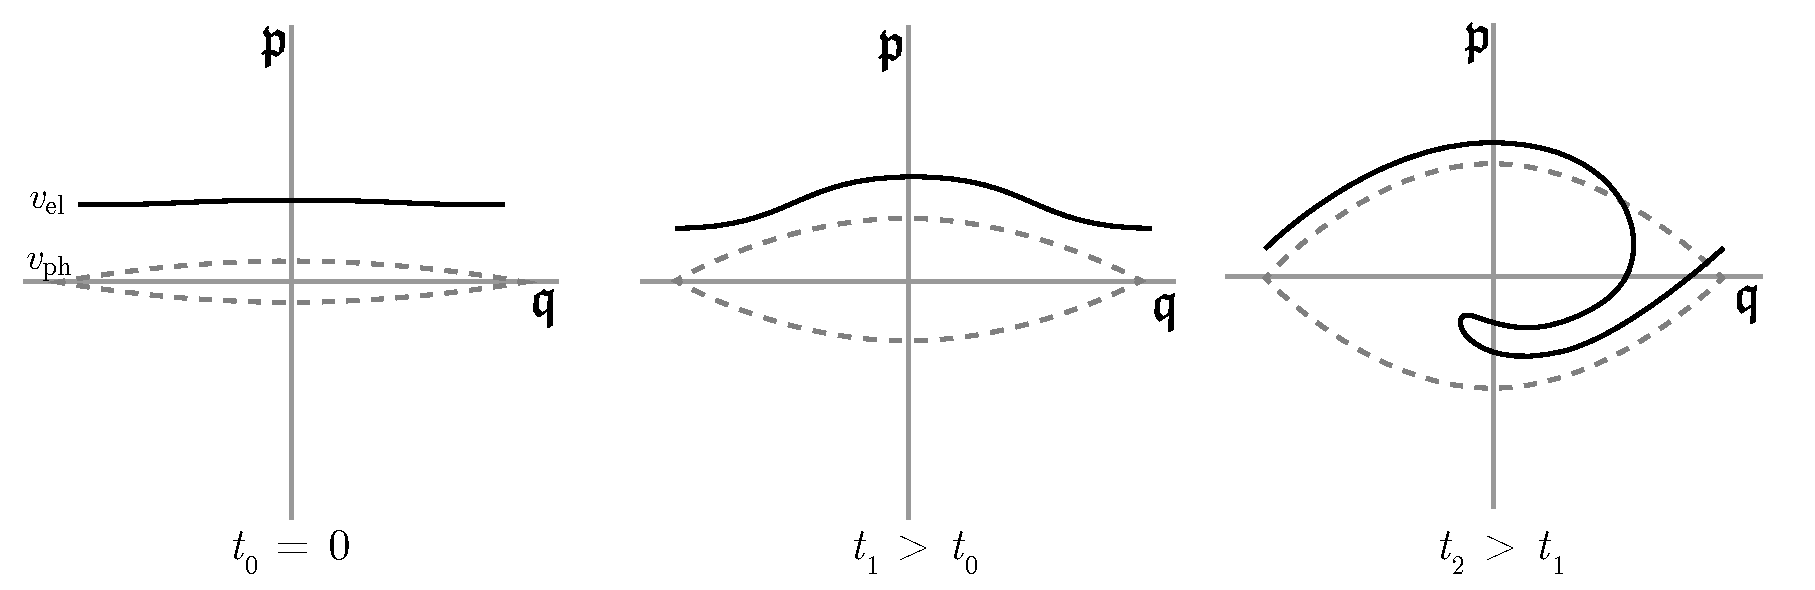
\includegraphics[width=1\textwidth]{Figs/Fig_cat_eyes_amplified.pdf}}
\end{figure}

\lipsum[4-7]

\begin{theorem}[Lipsum]
Donec et mi. Nam vulputate metus eu enim. Vestibulum pellentesque felis eu massa.
\end{theorem}

\begin{table}
\floatbox[{\capbeside\thisfloatsetup{capbesideposition={right,bottom},capbesidewidth=0.3\textwidth}}]{table}[\FBwidth]
{\caption{ \label{table1} Lorem ipsum dolor sit amet, consectetuer adipiscing elit. Ut purus elit, vestibulum ut, plac- erat ac, adipiscing vitae, felis. Curabitur dictum gravida mauris. Nam arcu libero, nonummy eget, consectetuer id, vulputate a, magna. Donec vehicula augue eu neque. Pellentesque habitant morbi tristique senectus et netus et malesuada fames ac turpis egestas. Mauris ut leo. }}%
{\hspace{-12mm} \begin{tabular}{|c|c|c||c|}
\hline
\textbf{IUT}                                                                                                       & \textbf{IEEE}       & \textbf{Frequency}        & \textbf{Used for}                                                                                                                                                                     \\ \hline
\hline
\multirow{3}{*}{\begin{tabular}[c]{@{}c@{}}High frequency\\ {\small Dekametric waves}\\    \end{tabular}}                  & \multirow{3}{*}{\textbf{HF}} & \multirow{3}{*}{3-30 MHz} & \multirow{3}{*}{\begin{tabular}[c]{@{}c@{}}Shortwave broadcasting, amateur\\  radio, over-the-horizon radio\\  (reflected off the ionosphere)\end{tabular}}                             \\
                                                                                                                   &                     &                           &                                                                                                                                                                                       \\
                                                                                                                   &                     &                           &                                                                                                                                                                                       \\ \hline
\begin{tabular}[c]{@{}c@{}}Very high freq.\\ {\small Metric waves}\end{tabular}                                         & \textbf{VHF}                 & 30-300 MHz                & FM and TV broadcasting                                                                                                                                                                \\ \hline
%                                                                                                                   &                     &                           &                                                                                                                                                                                       \\ \hline
\multirow{3}{*}{\begin{tabular}[c]{@{}c@{}}Ultra high freq.\\ {\small Decimetric waves}\\ 0.3-3 GHz\end{tabular}}       & \textbf{UHF}                 & 0.3-1 GHz              & \multirow{12}{*}{\begin{tabular}[c]{@{}c@{}}TV broadcasting,\\ microwave communication,\\ modern radars, \\ direct-broadcast satellite (DBS), \\ radio astronomy,\\ mobile phone,\\ wifi, bluetooth,\\ GPS, satellite radio\end{tabular}} \\ \cline{2-3}
                                                                                                                   & \textbf{L}                   & 1-2 GHz                   &                                                                                                                                                                                       \\ \cline{2-3}
                                                                                                                   & \multirow{2}{*}{\textbf{S}}  & \multirow{2}{*}{2-4 GHz}  &                                                                                                                                                                                       \\ \cline{1-1}
\multirow{5}{*}{\begin{tabular}[c]{@{}c@{}}Super high freq.\\ {\small Centimetric waves}\\ 3-30 GHz\end{tabular}}       &                     &                           &                                                                                                                                                                                       \\ \cline{2-3}
                                                                                                                   & \textbf{C}                   & 4-8 GHz                   &                                                                                                                                                                                       \\ \cline{2-3}
                                                                                                                   & \textbf{X}                   & 8-12 GHz                  &                                                                                                                                                                                       \\ \cline{2-3}
                                                                                                                   & \textbf{Ku}                  & 12-18 GHz                 &                                                                                                                                                                                       \\ \cline{2-3}
                                                                                                                   & \textbf{K}                   & 18-27 GHz                 &                                                                                                                                                                                       \\ \cline{1-3}
\multirow{4}{*}{\begin{tabular}[c]{@{}c@{}}Extremely high freq.\\ {\small Millimetric waves}\\ 30-300 GHz\end{tabular}} & \textbf{Ka}                  & 27-40 GHz                 &                                                                                                                                                                                       \\ \cline{2-3}
                                                                                                                   & \textbf{V}                   & 40-75 GHz                 &                                                                                                                                                                                       \\ \cline{2-3}
                                                                                                                   & \textbf{W}                   & 75-110 GHz                &                                                                                                                                                                                       \\ \cline{2-3}
                                                                                                                   & \textbf{mm} (G)            & 0.11-0.3 THz               &                                                                                                                                                                                       \\ \hline
\multicolumn{2}{|l|}{\multirow{2}{*}{\begin{tabular}[c]{@{}l@{}}Tremendously high freq.\\ {\small Sub-millimetric / Far infrared}\end{tabular}}} & \multirow{2}{*}{0.3-3 THz} & \multirow{2}{*}{\begin{tabular}[c]{@{}l@{}}Condensed-matter physics,\\ terahertz communication \end{tabular}} \\
\multicolumn{2}{|l|}{}                                                               &                    &                                                                \\ \hline
\end{tabular}}
\end{table}

\section{Another section}

Fusce mauris. Vestibulum luctus nibh at lectus. Sed bibendum, nulla a faucibus semper, leo velit ultricies tellus, ac venenatis arcu wisi vel nisl. Vestibulum diam. Aliquam pellen- tesque, augue quis sagittis posuere, turpis lacus congue quam, in hendrerit risus eros eget felis. Maecenas eget erat in sapien mattis porttitor. Vestibulum porttitor. Nulla facilisi. Sed a turpis eu lacus commodo facilisis. Morbi fringilla, wisi in dignissim interdum, justo lectus sagittis dui, et vehicula libero dui cursus dui. Mauris tempor ligula sed lacus. Duis cursus enim ut augue. Cras ac magna. Cras nulla. Nulla egestas. Curabitur a leo. Quisque egestas wisi eget nunc. Nam feugiat lacus vel est. Curabitur consectetuer.
Suspendisse vel felis. Ut lorem lorem, interdum eu, tincidunt sit amet, laoreet vitae, arcu. Aenean faucibus pede eu ante. Praesent enim elit, rutrum at, molestie non, nonummy vel, nisl. Ut lectus eros, malesuada sit amet, fermentum eu, sodales cursus, magna. Donec eu purus. Quisque vehicula, urna sed ultricies auctor, pede lorem egestas dui, et convallis elit erat sed nulla. Donec luctus. Curabitur et nunc. Aliquam dolor odio, commodo pretium, ultricies non, pharetra in, velit. Integer arcu est, nonummy in, fermentum faucibus, egestas vel, odio.



\subsection{Another subsection}

Fusce mauris. Vestibulum luctus nibh at lectus. Sed bibendum, nulla a faucibus semper, leo velit ultricies tellus, ac venenatis arcu wisi vel nisl. Vestibulum diam. Aliquam pellen- tesque, augue quis sagittis posuere, turpis lacus congue quam, in hendrerit risus eros eget felis. Maecenas eget erat in sapien mattis porttitor. Vestibulum porttitor. Nulla facilisi. Sed a turpis eu lacus commodo facilisis. Morbi fringilla, wisi in dignissim interdum, justo lectus sagittis dui, et vehicula libero dui cursus dui. Mauris tempor ligula sed lacus. Duis cursus enim ut augue. Cras ac magna. Cras nulla. Nulla egestas. Curabitur a leo. Quisque egestas wisi eget nunc. Nam feugiat lacus vel est. Curabitur consectetuer.
\begin{equation}
v_{{\rm el},0} = \sqrt{2 \eta V_0} \, , \label{velocity}
\end{equation}
Suspendisse vel felis. Ut lorem lorem, interdum eu, tincidunt sit amet, laoreet vitae, arcu. Aenean faucibus pede eu ante. Praesent enim elit, rutrum at, molestie non, nonummy vel, nisl. Ut lectus eros, malesuada sit amet, fermentum eu, sodales cursus, magna. Donec eu purus. Quisque vehicula, urna sed ultricies auctor, pede lorem egestas dui, et convallis elit erat sed nulla. Donec luctus. Curabitur et nunc. Aliquam dolor odio, commodo pretium, ultricies non, pharetra in, velit. Integer arcu est, nonummy in, fermentum faucibus, egestas vel, odio.

\begin{itemize}
\item[\textcolor{QuarkColor}{$\diamond$}]  Ut lorem lorem, interdum eu, tincidunt sit amet, laoreet vitae, arcu. Aenean faucibus pede eu ante. 
\item[\textcolor{QuarkColor}{$\diamond$}]  Ut lorem lorem, interdum eu, tincidunt sit amet, laoreet vitae, arcu. Aenean faucibus pede eu ante. 
\item[\textcolor{QuarkColor}{$\diamond$}]  Ut lorem lorem, interdum eu, tincidunt sit amet, laoreet vitae, arcu. Aenean faucibus pede eu ante. Ut lorem lorem, interdum eu, tincidunt sit amet, laoreet vitae, arcu. Aenean faucibus pede eu ante. 
\end{itemize}




